\documentclass[a4paper,12pt]{report}
% safe参数解决与\!在内的多个冲突
% \sups命令可能被重定义,xeCJK放在tipa后
\usepackage[safe]{tipa}
\usepackage{algorithm}
\usepackage{amsmath,bm}
\usepackage{algorithmic}
\usepackage{fancybox}
\usepackage{listings}
\usepackage{xcolor}
\usepackage{diagbox}
\usepackage{amssymb}
\usepackage{amsmath}
\usepackage{amsthm}
\usepackage{empheq}
\usepackage[framemethod=tikz]{mdframed}
\usepackage{mathtools}

\definecolor{ocre}{RGB}{243,102,25}
\definecolor{mygray}{RGB}{243,243,244}

\newcommand*\mymathbox[1]{%
  \fcolorbox{ocre}{mygray}{\hspace{1em}#1\hspace{1em}}}

\newtheoremstyle{mystyle}
  {\topsep}
  {\topsep}
  {\normalfont}
  {}
  {\sffamily\bfseries}
  {.}
  {.5em}
  {{\color{ocre}\thmname{#1}~\thmnumber{#2}}\thmnote{\,--\,#3}}%
\theoremstyle{mystyle}
\newmdtheoremenv[
  backgroundcolor=mygray,
  linecolor=ocre,
  leftmargin=20pt,
  innerleftmargin=0pt,
  innerrightmargin=0pt,
  ]{theo}{Theorem}[section]

\lstset{
columns=flexible,
numbers=left,
numberstyle=\footnotesize\color{darkgray}, 
basicstyle=\small\ttfamily,
stringstyle=\color{purple},
keywordstyle=\color[RGB]{40,40,255}\bfseries,
commentstyle=\it\color[RGB]{0,96,96},  
stringstyle=\rmfamily\slshape\color[RGB]{128,0,0}, 
showstringspaces=false,      
% directivestyle=\color{blue},
frame=shadowbox,
%framerule=0pt,
backgroundcolor=\color[RGB]{245,245,244},
escapeinside=``, %逃逸字符(1左面的键),用于显示中文
breaklines,
extendedchars=false,
%解决代码跨页时,章节标题,页眉等汉字不显示的问题
xleftmargin=2em,xrightmargin=2em,
aboveskip=1em,%设置边距
tabsize=4, %设置tab空格数  
showspaces=false %不显示空格 
rulesepcolor=\color{red!20!green!20!blue!20}
%rulesepcolor=\color{brown}
}
% 中文支持
\usepackage[slantfont,boldfont]{xeCJK}
	\setCJKmainfont[BoldFont=SimHei,ItalicFont=KaiTi]{SimSun}
	\setCJKmathfont{STXinwei}
\usepackage{indentfirst}

% 数学环境
\usepackage{amsmath}
  \newcommand{\ue}{\mathrm{e}}
  \newcommand{\ud}{\mathop{}\negthinspace\mathrm{d}}
\usepackage{amssymb}
\usepackage{mathrsfs} % 线性代数字体
    % overline的替代命令
\newcommand{\closure}[2][3]{{}\mkern#1mu\overline{\mkern-#1mu#2}}
\usepackage{yhmath} % 左下-右上省略号
\usepackage{mathtools} % dcases环境
\usepackage{amsthm} % 定理环境
  \theoremstyle{definition}\newtheorem{laws}{Law}[section]
  \theoremstyle{plain}\newtheorem{ju}[laws]{Jury}
  \theoremstyle{remark}\newtheorem*{marg}{Margaret}
\usepackage{esint} % 多重积分,需放在amsmath后

% 下划线宏包
\usepackage{ulem}
% LaTeX符号宏包
\usepackage{hologo}
	\newcommand{\xelatex}{\Hologo{XeLaTeX}}
	\newcommand{\bibtex}{\Hologo{BibTeX}}
% 其他符号
\usepackage{wasysym}
% 带箱小页
\usepackage{boxedminipage}
% 绘图
\usepackage{tikz}
	\usetikzlibrary{calc}
	\newcommand{\tikzline}[1]{{#1\tikz{\draw[#1,line width=9](0,0)--(0.5,0);}}, }

% 奇怪的小定义
\newcommand{\dpar}{\\ \mbox{}}	% 空两行
\newcommand{\qd}[1]{{\bfseries{#1}}}	% 强调
\newcommand{\co}[1]{{\bfseries{#1}}}   % Style of concept
\newcommand{\RED}[1]{{\color{red}{#1}}}
\newcommand{\cmmd}[1]{\fbox{\texttt{\char92{}#1}}}
\newcommand{\charef}[1]{第\ref{#1}章}
\newcommand{\secref}[1]{第\ref{#1}节}
\newcommand{\pref}[1]{第\pageref{#1}页}
\newcommand{\fref}[1]{图\ref{#1}}
\newcommand{\tref}[1]{表\ref{#1}}

% 编号列表宏包,并自定义了三个列表
%\usepackage[inline]{enumitem}
%	\setlist[enumerate]{label=\arabic* - ,font=\bfseries,itemsep=0pt}
%	\setlist[itemize]{label=$\bullet$,font=\bfseries,leftmargin=\parindent}
%	\setlist[description]{font=\bfseries\uline}
%
%\newenvironment{fead}{\setlength{\parskip}{0pt}
%	\begin{description}[font=\bfseries\uline,labelindent=\parindent]
%		\setlength{\itemsep}{0pt}\setlength{\parsep}{0pt}\setlength{\parskip}{0pt}}
%	{\end{description}}
% 带宽度的
\newenvironment{para}{\setlength{\parskip}{0pt}
	\begin{description}[font=\bfseries\ttfamily]
		\setlength{\itemsep}{0pt}\setlength{\parsep}{0pt}\setlength{\parskip}{0pt}}
	{\end{description}}
\newenvironment{feae}{\setlength{\parskip}{0pt}
	\begin{enumerate}[font=\bfseries,labelindent=0pt]}
	{\end{enumerate}}
\newenvironment{feai}{\setlength{\parskip}{0pt}
	\begin{itemize}[font=\bfseries]
		\setlength{\itemsep}{0pt}\setlength{\parsep}{0pt}\setlength{\parskip}{0pt}}
	{\end{itemize}}
\newenvironment{inlinee}
{\begin{enumerate*}[label=(\arabic*), font=\rmfamily, before=\unskip{:},itemjoin={{;}},itemjoin*={{,以及:}}]}
	{\end{enumerate*}。}

% 目录和章节样式
\usepackage{titlesec}
\usepackage{titletoc}   % 用于目录

\titlecontents{chapter}[1.5em]{}
	{\contentslabel{1.5em}}{\hspace*{-2em}}{\hfill\contentspage}
	
\titlecontents{section}[3.3em]{}
	{\contentslabel{1.8em}}
	{\hspace*{-2.3em}}
	{\titlerule*[8pt]{$\cdot$}\contentspage}
%	
\titlecontents{subsection}[2.5em]{\small}
	{\thecontentslabel{} }
	{}
	{\titlerule*[5pt]{$\cdot$}\contentspage}
 %章节样式
\setcounter{secnumdepth}{3} % 一直到subsubsection
\newcommand{\chaformat}[1]{%
	\parbox[b]{.5\textwidth}{\hfill\bfseries #1}%
	\quad\rule[-12pt]{2pt}{70pt}\quad
	{\fontsize{60}{60}\selectfont\thechapter}}
\titleformat{\chapter}[block]{\hfill\LARGE\sffamily}{}{0pt}{\chaformat}[\vspace{2.5pc}\large
	\startcontents\printcontents{}{1}{\setcounter{tocdepth}{2}}]
%\titleclass{\section}{top}
%\titleformat{\section}{\Large\bfseries}{\thesection}{0.5em}{}
\titleformat*{\section}{\centering\Large\bfseries}
\titleformat{\subsubsection}[hang]{\bfseries\large}{\rule{1.5ex}{1.5ex}}{0.5em}{}
% 扩展章节
\newcommand{\starsec}{\noindent\fbox{\S\textit{注意:本章节是一个扩展阅读章节。}}
	\\ \mbox{}}

\renewcommand{\contentsname}{目录}
	\renewcommand{\tablename}{表}
	\renewcommand\arraystretch{1.2}	% 表格行距
	\renewcommand{\figurename}{图}
% 设置不需要浮动体的表格和图像标题
\setlength{\abovecaptionskip}{5pt}
\setlength{\belowcaptionskip}{3pt}
\makeatletter
\newcommand\figcaption{\def\@captype{figure}\caption}
\newcommand\tabcaption{\def\@captype{table}\caption}
\makeatother
% 图表
\usepackage{array,multirow}
  \setlength\extrarowheight{2pt} % 行高增加
\usepackage{longtable}
\usepackage{graphicx}
  \graphicspath{{./tikz/}}
% 页面修正宏包
\usepackage[top=1in]{geometry}

% 代码环境
\usepackage{listings}
% Avoid copy line numbers of the listing code (Invalid for SumatraPDF Reader)
\usepackage{accsupp}
	\newcommand{\emptyaccsupp}[1]{\BeginAccSupp{ActualText={}}#1\EndAccSupp{}}
% Color
\usepackage{xcolor}
	\definecolor{commentcolor}{RGB}{85,139,78}
	\definecolor{numbercolor}{RGB}{166,206,168}
	\definecolor{stringcolor}{RGB}{206,145,108}
	\definecolor{keywordcolor}{RGB}{34,34,250}
	\definecolor{backcolor}{RGB}{220,220,220}
	\definecolor{packagecolor}{RGB}{0,128,0}
	\definecolor{envicolor}{RGB}{185,70,15}
% LaTeX Code Style
%\lstset{language=[LaTeX]TeX,
%		basicstyle=\small\ttfamily,
%		commentstyle=\color{commentcolor},
%		keywordstyle=\color{keywordcolor},
%		stringstyle=\color{stringcolor},
%		showstringspaces=false,
%		% Package/Tikz-Lib Using
%		classoffset=0,
%		morekeywords={begin,end,usetikzlibrary},
%		keywordstyle=\color{keywordcolor},
%		classoffset=1,
%		morekeywords={article,report,book,
%			xeCJK,tikz,
%			calc},
%		keywordstyle=\color{packagecolor},
%		classoffset=2,
%		morekeywords={document,tikzpicture},
%		keywordstyle=\color{envicolor},
%		% Line Number Style
%		numbers=left,
%		numberstyle=\tiny\emptyaccsupp,
%		stepnumber=1,
%		% Frame and Background Color
%		frame=single,
%		framerule=0pt,
%		backgroundcolor=\color{backcolor},
%		% Spaces
%		% belowskip=\medskipamount,
%		emptylines=1,
%		escapeinside=``}

\lstnewenvironment{latex}[1]{\lstset{#1}}{}
\newcommand{\latexline}[1]{{\lstinline[language=TeX,basicstyle=\small\ttfamily]{#1}}}

% Tikz Code
\lstdefinelanguage{tikzlang}{
	classoffset=0, % 蓝色的keyword
	morekeywords={begin,end,newcommand,
		draw,node,coordinate,tikzstyle,foreach},
	keywordstyle=\color{keywordcolor},
	classoffset=1, % 棕色的其他关键字
	morekeywords={tikzpicture,grid,at,
		thick,thin,very,ultra,
		red,green,yellow,blue,cyan,magenta,black,
		    gray,darkgray,lightgray,brown,lime,
		    olive,orange,pink,purple,teal,violet,white},
	keywordstyle=\color{envicolor},
	morecomment=[l]{\%},
	morecomment=[s]{/*}{*/},
	morestring=[b]',
	% Escape
	escapeinside=``
}
\lstnewenvironment{tikzcode}[1]{\lstset{language=tikzlang,basicstyle=\small\ttfamily,
		breaklines=true,%backgroundcolor=\color{white},
		linewidth=0.7\linewidth,#1}}{}

% 附录
\usepackage{appendix}

% 行号
\usepackage{lineno}

% 代码输入环境
%\usepackage{verbatim,xcolor}
%\newbox\savedlines
%\newtoks\savedtokens
%\makeatletter
%\def\codeshow{%
%\global\savedtokens={}%
%\def\verbatim@processline{%
%{\setbox0=\hbox{\the\verbatim@line}%
%\hsize=\wd0
%\the\verbatim@line\par}%
%\global\savedtokens=\expandafter{\the\expandafter\savedtokens\the\verbatim@line^^J}}%
%\@tempswatrue
%\setbox0=\vbox\bgroup\parskip=0pt\topsep=0pt\partopsep=0pt
%\verbatim}
%\def\endcodeshow{\endverbatim%
%\unskip\setbox0=\lastbox\egroup
%\global\setbox\savedlines=\box0
%\addvspace{1em}\par\noindent%
%\colorbox{lightgray}{%
%\begin{minipage}{.55\textwidth}{\usebox\savedlines}\end{minipage}}%
%\hfill\fbox{\parbox{.40\textwidth}%
%{\scantokens\expandafter{\the\savedtokens\unskip\endinput}}}%
%\par\addvspace{1em}}
%\makeatother

% 引用
\usepackage[colorlinks,bookmarksopen=true,bookmarksnumbered=true]{hyperref}

\renewcommand{\algorithmicrequire}{ \textbf{Input:}} %Use Input in the format of Algorithm  
\renewcommand{\algorithmicensure}{ \textbf{Output:}} %UseOutput in the format of Algorithm  


\title{神经网络和深度学习笔记}
\author{张晋\\北京航空航天大学\\数学与系统科学学院}
\date{最后更新于:\today}
\begin{document}

\maketitle

\tableofcontents


\newpage

\chapter{神经网络简介}
\textit{“神经网络是由具有适应性的简单单元组成的广泛并行互连的网络,它的组织能够模拟生物神经系统对真实世界物体所作出的交互反应”}---[Kohonen,1988]

\newpage
\section{生物神经网络(Biological Neural Networks)}
大脑可视作为1000多亿神经元组成的神经网络。

神经元的信息传递和处理是一种电化学活动.树突由于电化学作用接受外界的刺激;通过胞体内的活动体现为轴突电位,\textcolor{red}{当轴突电位达到一定的值则形成神经脉冲或动作电位};再通过轴突末梢传递给其它的神经元.从控制论的观点来看;这一过程可以看作一个\textcolor{red}{多输入单输出非线性}系统的动态过程。


\begin{figure}[h]
\small
\centering
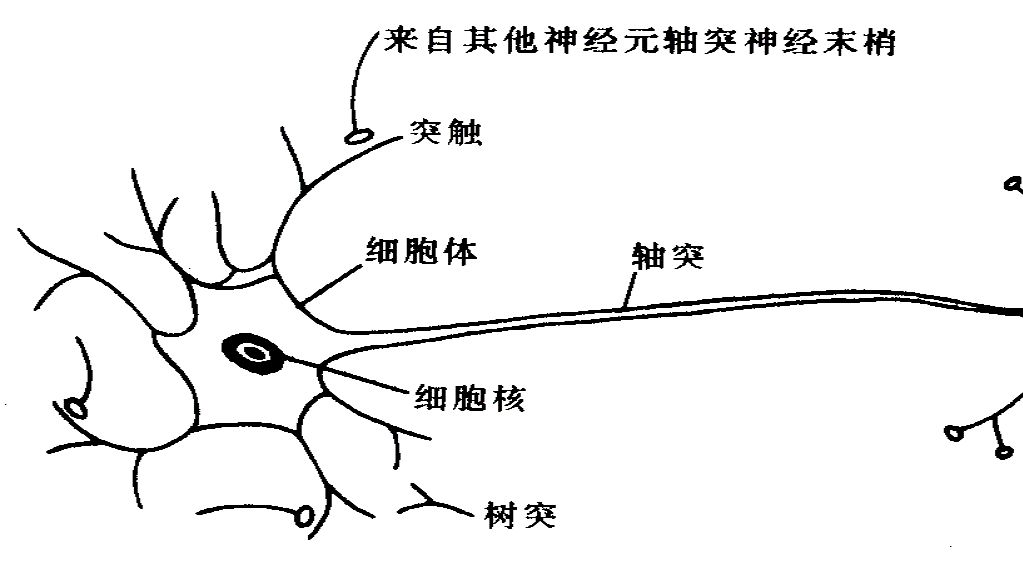
\includegraphics[width=14cm]{figure//1.png}
\caption{神经元信息的传递} \label{fig:1}
\end{figure}


\subsection*{大脑处理信息的特点}
\begin{itemize}
\item \textbf{分布存储与冗余性}: 记忆在大量元中,每个元存在许多信息的部分内容,信息在神经网络中的记忆反映在神经元间的突触连接强度上

\item \textbf{并行处理}: 经网络既是处理器又是存储器(并行处理不同于并行机)

\item \textbf{信息处理与存储合一}: 每个元兼有二者功能

\item \textbf{可塑性与自组织性}: 可塑性是学习记忆的基础

\item \textbf{鲁棒性}: 高连接度导致一定的误差和噪声不会使网络性能恶化。是智能演化的重要因素

\end{itemize}

\newpage
\section{人工神经网络(Artificial Neural Networks)
}
神经网络是一个并行和分布式的信息处理网络结构,它一般由许多个神经元组成,每个神经元只有一个输出,它可以连接到很多其他的神经元,每个神经元输入有多个连接通道,每个连接通道对应于一个连接权系数。

\begin{figure}[h]
\small
\centering
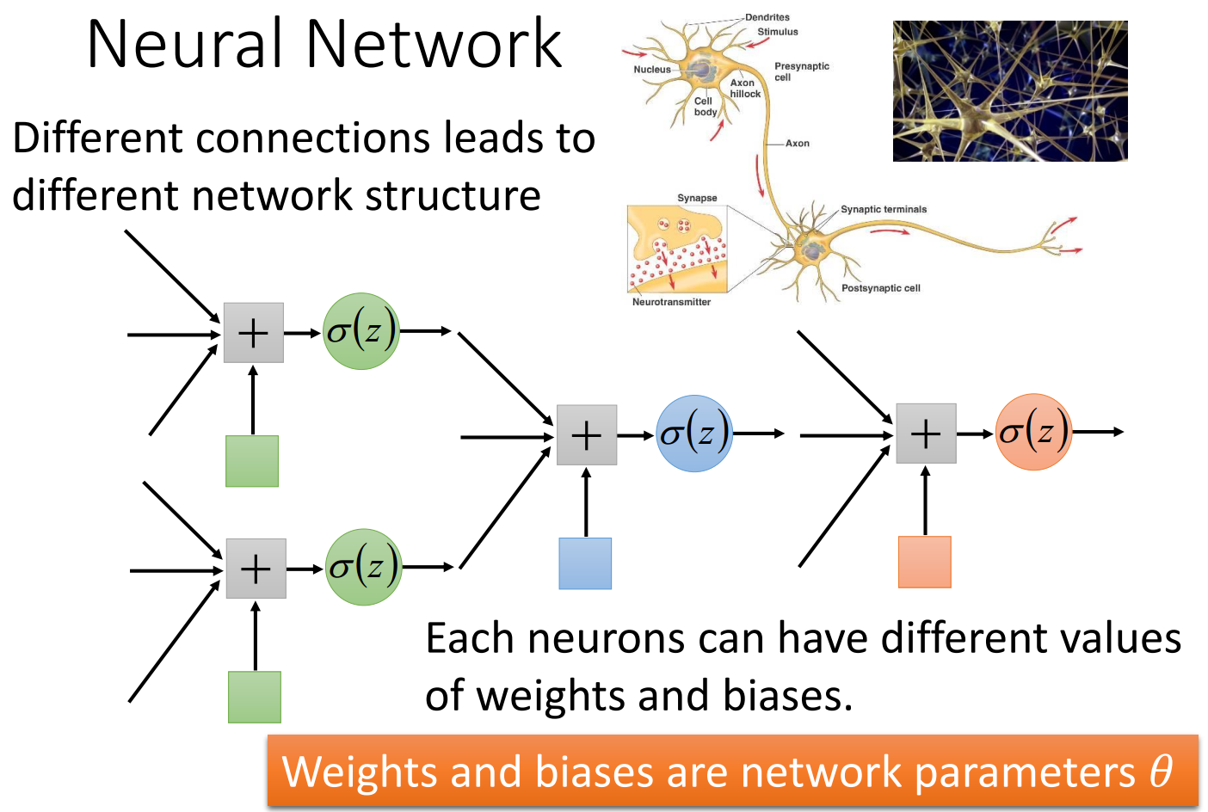
\includegraphics[width=16cm]{figure//2.png}
\caption{Artificial Neural Networks} \label{fig:2}
\end{figure}

\subsection{人工神经元模型(Artificial Neuron Model)}

神经网络中最基本的成分是\textcolor{blue}{神经元(neuron)模型},即上述定义中的“简单单元”。在生物神经网络中,每个神经元与其他神经元相连,当它“兴奋”时,就会向相连的神经元发送化学物质,从而改变这些神经元内的电位;如果某神经元的电位超过了一个\textcolor{blue}{"阈值”(threshold)},那么它就会被激活,即“兴奋"起来,向其他神经元发送化学物质。

1943年,[Mccu11ochandPitts,1943]将上述情形抽象为图所示的简单模型,这就是一直沿用至今的“M-P神经元模型”在这个模型中,神经元接收到来自n个其他神经元传递过来的输入信号,这些输入信号通过带权重的连接(connection)进行传递,神经元接收到的总输入值将与神经元的阈值进行比较然后通过\textcolor{blue}{“激活函数”(activation function)}处理已产生神经元的输出。

\begin{figure}[h]
\small
\centering
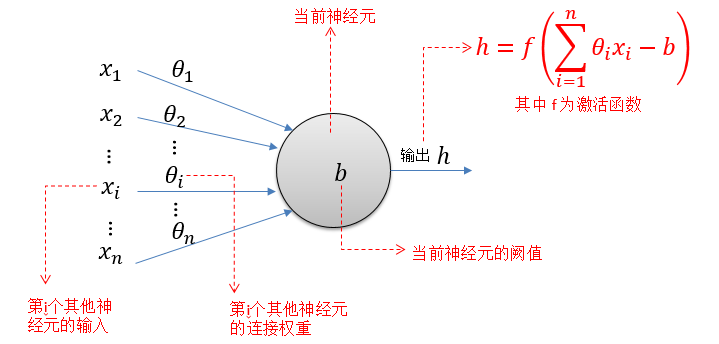
\includegraphics[width=14cm]{figure//3.png}
\caption{Artificial Neuron Model} \label{fig:3}
\end{figure}

\subsection*{激活函数}
理想中的激活函数$f(x)$是图(a)所示的阶跃函数,它将输入值映射为输出值“0”或“1”,“1”对应神经元兴奋,“0”对应神经元抑制。但是,阶跃函数具有不连续,不光滑(不连续可导)等不太好的性质\footnote{事实上在使用阶跃函数时,神经网络中的权值或偏置的微小改变可能会造成输出结果天翻地覆的变化,这使得网络的行为变得复杂且难以控制。},因此实际中常用Logistic回归中应用到的\textcolor{blue}{sigmoid函数}作为激活函数。典型的sigmoid函数如图(b)所示,它把可能在较大范围内变化的输入值挤压到(0,1)输出值范围内,因此有时又称之为“挤压函数”(squashing function).

\begin{figure}[h]
\small
\centering
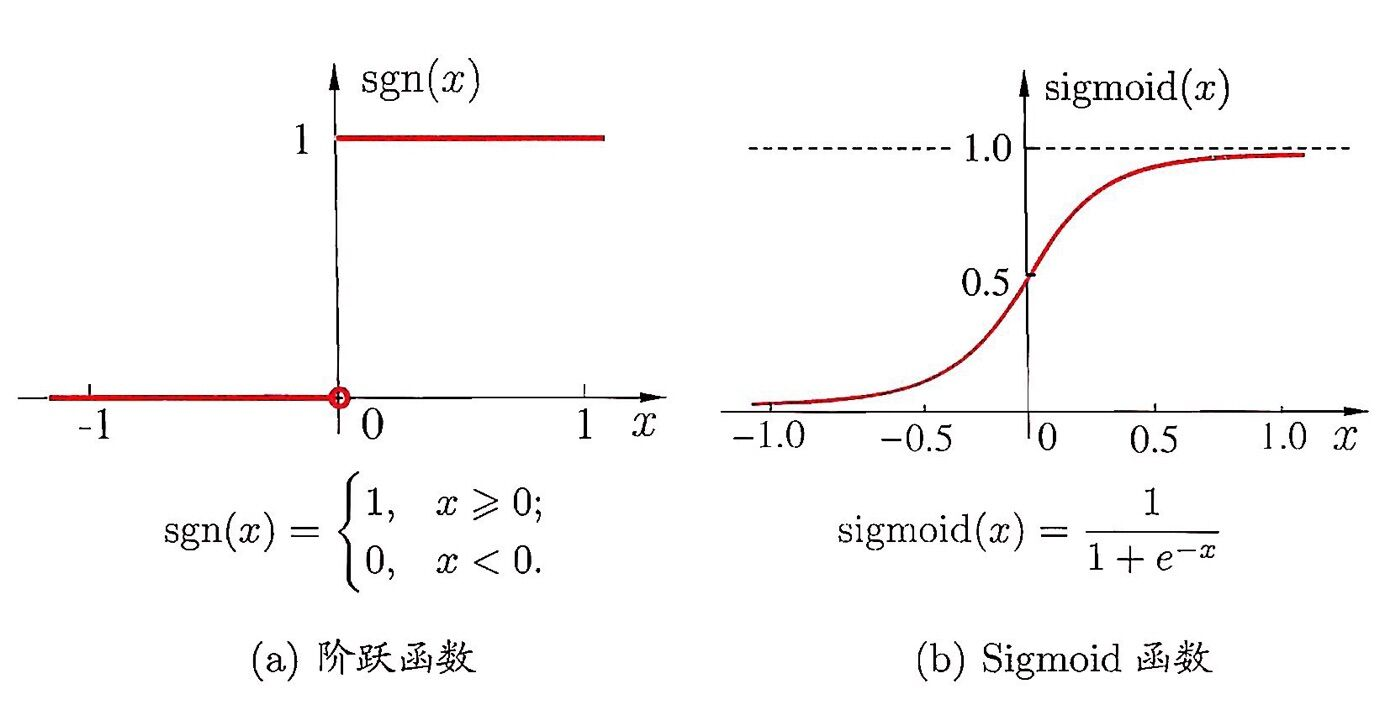
\includegraphics[width=14cm]{figure//4.jpg}
\caption{激活函数} \label{fig:4}
\end{figure}


\subsection{人工神经网络的构成(Structure of ANN)}
\subsubsection{感知机(Perceptron)}

感知机(Perceptron)由两层神经元组成,如图所示,输入层接收外界输入信号后传递给输出层,输出层是M-P神经元,亦称"阈值逻辑单元"(threshold logic unit)

感知器处理单元对$n$个\textbf{二进制}输入$x_1,x_2,\ldots$,进行加权和操作并产生一个二进制输出:
\[\boxed{y=f\big(\sum_i w_ix_i-\theta\big)}\]

感知机能容易地实现逻辑\textbf{与、或、非}运算:

\begin{itemize}

\item 先定义$f(x)$为阶跃函数

\item “与”$(x_1\wedge x_2)$: 
令$w_1=w_2=1,\theta=2$;
则仅在$x_1=x_2=1$时,$y=1$;

\item “或”$(x_1\vee x_2)$: 
令$w_1=w_2=1,\theta=0.5$;
则仅在$x_1=x_2=1$时,$y=1$;

\item “非”$(\neg x_1)$: 
令$w_1=-0.6,w_2=0,\theta=-0.5$;
那么当$x_1=1$时,$y=0$;
\end{itemize}

\begin{figure}[h]
\small
\centering
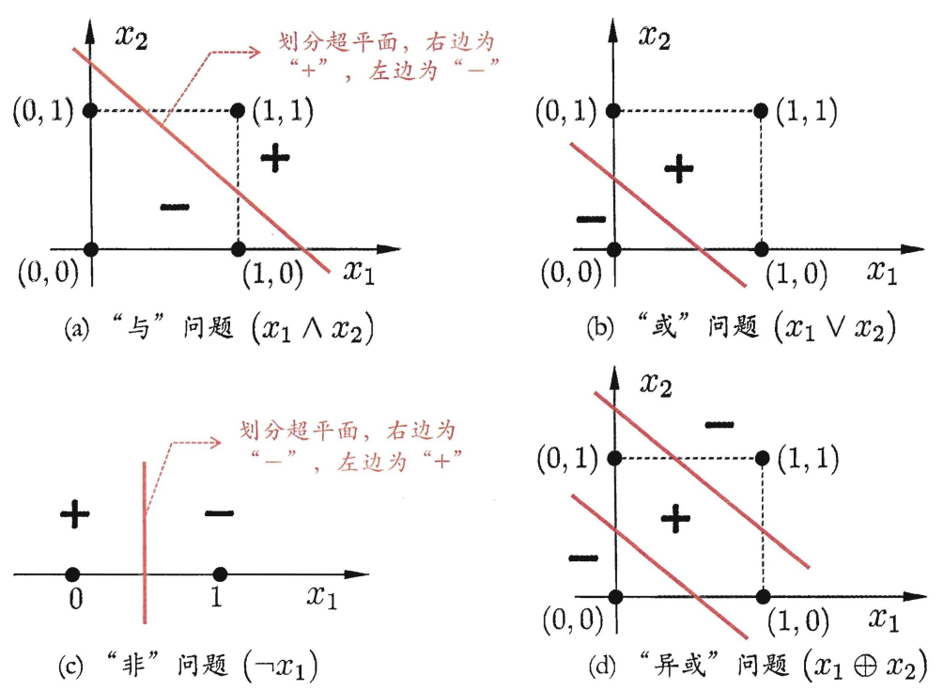
\includegraphics[width=14cm]{figure//5.png}
\caption{与、或、非运算的实现} \label{fig:5}
\end{figure}

需注意的是,感知机只有输出层神经元进行激活函数处理,即只拥有一层功能神经元 (functional neuron),其学习能力非常有限,只能处理\textcolor{red}{线性可分(linearly separable)}的问题。

从图中可以看出,与、或、非问题的分类样本是可以用一条直线分开的,即具有“线性可分”性质。



\subsubsection{多层感知机(MLP)}

\textcolor{red}{要解决非线性可分问题,就需考虑多层功能神经元。}

而“异或”问题的分类样本需要两条线才能将其分开,故需要两层感知机才能实现,如图1.6

\begin{figure}[h]
\small
\centering
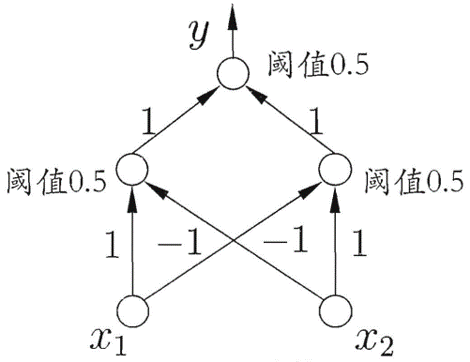
\includegraphics[width=6cm]{figure//6.png}
\caption{能解决异或问题的两层感知机} \label{fig:6}
\end{figure}

多层感知机(MLP)的结构如下:
\begin{center}
  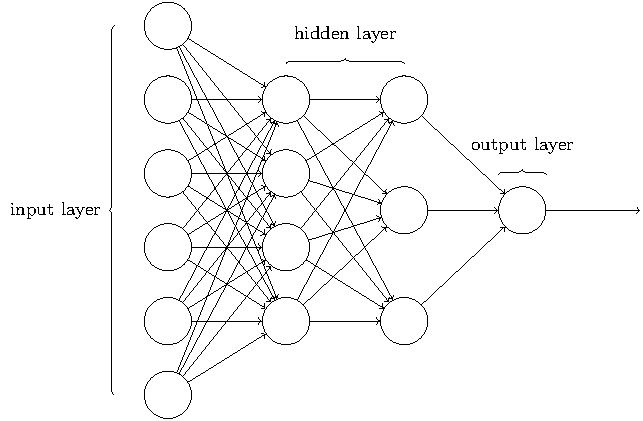
\includegraphics{figure//tikz11}
\end{center}

\begin{itemize}
\item 这个网络中最左边的称为\textbf{输入层},其中的神经元称为\textbf{输入神经元}。

\item 最右边的,即\textbf{输出层}包含有\textbf{输出神经元}。

\item 中间层,这层中的神经元既不是输入也不是输出,被称为\textbf{隐藏层}。 

\item 隐含层和输出层神经元都是拥有\textcolor{red}{激活函数}的功能神经元. 

\item 只需包含隐层,即可称为多层网络.神经网络的学习过程,就是根据训练数据来调整神经元之间的\textcolor{blue}{“连接权” (connection weight)}以及每个功能神经元的阈值;

\item 换言之,神经网络“学”到的东西,蕴涵在\textcolor{red}{连接权}与\textcolor{red}{阈值}中。

\end{itemize}
\subsection{人工神经网络的学习(Training of ANN)}
\textcolor{blue}{\textbf{反向传播算法}(error Back Propagation,简称 BP)}是迄今最成功的神经网络学习算法.它可用来学习由一系列确定的单元互连形成的多层网络的权值。
它采用\textcolor{red}{梯度下降方法}试图最小化网络输出值和目标值之间的\textcolor{blue}{误差平方}。
其主要思想是:
\begin{enumerate}
\item 将训练集数据输入到ANN的输入层,经过隐藏层,最后达到输出层并输出结果,这是ANN的前向传播过程;

\item 由于ANN的输出结果与实际结果有误差,则计算估计值与实际值之间的误差,并将该误差从输出层向隐藏层反向传播,直至传播到输入层;

\item 在反向传播的过程中,根据误差调整各种参数的值;不断迭代上述过程,直至收敛。

\begin{figure}[h]
\small
\centering
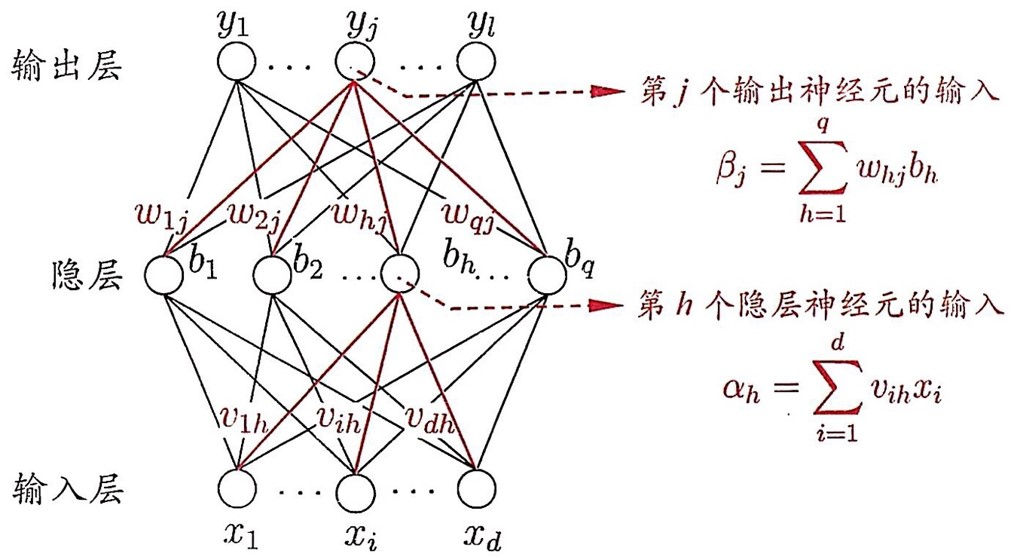
\includegraphics[width=14cm]{figure//7.jpg}
\caption{神经网络} \label{fig:7}
\end{figure}

\begin{algorithm}[h]  
\caption{BP Algorithm}  
\begin{algorithmic}[1]  
\REQUIRE ~~\\
训练集$D={(x_k,y_k)}_{k=1}^m$,学习率 $\eta$
\ENSURE ~~\\
连接权与阈值确定的多层前馈神经网络

\STATE 在(0,1)范固内随机初始化网络中所有连接权和阈值
\WHILE {未达到停止条件}
\STATE 计算当前样本的输出$\hat{y}_k$
\STATE 计算输出层神经元的梯度项$g_j$
\STATE 计算隐层神经元的梯度项 $e_h$
\STATE 更新连接权$w_{hj},v_{ih}$与阈值$\theta_j,\gamma_h$
\ENDWHILE
\end{algorithmic}  
\end{algorithm}  
\end{enumerate}

\section{神经网络应用现状}
人工神经网络(ANN)以其独特的结构和处理信息的方法,在许多实际应用领域中取得了显著的成效,主要应用如下:
\begin{itemize}
\item \textbf{模式识别}\\
\textit{在模式识别实践中通常存在着噪声干扰和输入输出信息缺失的情况,神经网络的分布式信息存储特性使得其具有良好的容错性和鲁棒性,因此在解决模式识别问题时具有较大的优越性。事实上,模式识别技术的广泛应用也是人工神经网络技术发展的一个重要方面。神经网络在这个领域中有许多成功的应用,例如目前市场上被人们广为熟知的手写输入和语音输入等智能系统。}

\item \textbf{自动控制}\\
\textit{神经网络的诸多特点决定了其应用于自动控制领域的优越性。如神经网络本质上就是并行计算、分布结构的非线性动力学系统,可应用于那些难以用模型描述的过程或系统及应用于实时性要求较高的自动控制领域。另外,神经网络具有较强的信息综合能力,在多变量复杂系统的控制方案设计上具有一定明显的优势。}

\item \textbf{信号处理}\\
\textit{    神经网络的自学习和自适应特性使其成为一种对各类信号进行多用途综合加工处理的天然工具,被广泛地应用于自适应信号处理和非线性信号处理。
}

\item \textbf{人工智能}\\
\textit{人们在应用专家系统解决类似于人脑形象思维的问题时遇到了较大的困难,而人工神经网络的发展则为本已遇到“瓶颈”问题的人工智能带来了新的出路。这主要得益于人工神经网络的自学习、自适应能力和良好的容错特性。这方面的主要应用有自然语言处理、逻辑推理、模糊判断、系统诊断、密码破译、智能机器人等。
}
\end{itemize}

以上只是大概地简单列举了四个方面的应用。事实上,人工神经网络的应用领域是十分广泛的。例如,人工神经网络还可以用来解决最优化问题(包括组合优化、条件约束优化等这类问题)或者开发出用于矩阵/向量运算的数字计算机协处理器,在经济领域中也可以用来进行市场预测和信贷分析等方面的工作。此外,在医学领域、军事领域、化学领域甚至娱乐视听领域,人工神经网络都取得了一定的成功应用。这也正是科学技术转化为具体生产力的表现。相信随着人工神经网络研究的进一步深人和发展,特别是当人工神经网络作为一种智能化方法同其他学科和领域更为紧密地结合起来的时候,人工神经网络的应用前景也将更为广阔。

\chapter{反向传播算法}
反向传播算法的核心是一个对代价函数 $C$ 关于任何权重 $w$
和偏置$b$的偏导数 $\partial C/\partial w,\partial C/\partial b$ 的表达式。这个表达式告诉我们在改变权重和偏置时,代价函数变化的快慢,所以反向传播不仅仅是一种学习的快速算法。实际上它让我们细致领悟如何通过改变权
重和偏置来改变整个网络的行为。



\end{document}